\documentclass[notitlepage,oneside]{book}
%Configuración
%\usepackage[utf8]{inputenc}
\usepackage[spanish,es-tabla]{babel} %opción es-tabla para que diga Tabla en vez de Cuadro
\usepackage{float} %Paquete para poder definir la posición de una tabla con "H"
\usepackage{booktabs} %Paquete para que las tablas se vean bonitas
\usepackage{tikz} %Paquete para hacer figuras
\usepackage{pgfplots} %Paquete para hacer gráficos
\pgfplotsset{compat=1.16} %Compatibilidad para gráficos
%\usepackage{cite}% Paquete para realizar citas
\usepackage{geometry}%Paquete utilizado provisionalmente para dar formato preliminar al documento
\geometry{left=35mm,right=20mm,top=30mm,bottom=30mm,headheight=15pt}
\usepackage{graphicx}
\usepackage{multirow}%Permite realizar configuracion multifila en tablas
\usepackage{gensymb}%Permite agregar el simbolo de grados %use \siunitx para eso
\usepackage{xurl}%Para hipervinculos
\usepackage[T1]{fontenc}
\usepackage[intoc, spanish]{nomencl}
\makenomenclature
\usepackage{appendix}
\usepackage{subfigure}
\usepackage{amsmath}
\usepackage{pdfpages}
%\usepackage{showlabels}
\usepackage{siunitx}\sisetup{add-arc-second-zero,output-decimal-marker = {,},number-unit-separator=\text{\,}}
\usepackage[colorlinks = true,
            linkcolor = blue,
            urlcolor  = blue,
            citecolor = blue,
            anchorcolor = blue]{hyperref}
\usepackage{textcomp}
%Comandos para darle formato a la hoja
%\geometry{width=15.5cm, marginpar=1cm}
\usepackage{tabularx}
\setlength{\parskip}{1.5mm}
\usepackage{lipsum}
\usepackage{float}  %poner tablas  e imagenes donde quiero
\usepackage{placeins}
\usepackage{amsmath, amsthm, amssymb} % para ecuaciones  %agregar funciones matemáticas
\usepackage{array}    %%tablas combinar columnas
\usepackage{multirow}  %tablas combinar filas
\usepackage{color}     %añadir color al texto
\usepackage{bookmark}
\begin{document}
%Páginas preliminares
\pagenumbering{roman}
\begin{titlepage}

\centering

{
\includegraphics[width=0.7\textwidth]{01_preliminares/00_figuras/logo.png}\par}
\vspace{0.5cm}

{\bfseries\LARGE Escuela de Ingeniería Electromecánica\par}
\vspace{0.5cm}



\vfill
%\vspace{1cm}

{\scshape\LARGE Título del proyecto \par}
\vspace{1cm}

{\itshape\Large Informe de Práctica de Especialidad para optar por el Título de
Ingeniero en Mantenimiento Industrial, Grado Licenciatura \par}
\vspace{1cm}

{\Large Autor: \par}
{\Large Nombres y Apellidos  \par}
\vspace{0.6cm}

{\Large Lugar, Mes Año \par}

\vspace{0.5cm}

{\Large Carrera Acreditada por: \par}
{
\includegraphics[width=0.4\textwidth]{01_preliminares/00_figuras/AAPIA.png}\par}



\end{titlepage}

\thispagestyle{plain}
\chapter*{Resumen}

\lipsum[4-6]

\textbf{Palabras Claves:} \lipsum[4][2], \lipsum[4][7], \lipsum[4][9]

\thispagestyle{plain}
\chapter*{Abstract}

\lipsum[1-3]

\textbf{Key Words:} \lipsum[4][2], \lipsum[4][7], \lipsum[4][9]


\thispagestyle{plain}
\chapter*{Agradecimientos}
\begin{flushright}
\textit{\lipsum[5][3]}
\end{flushright}
\vspace{1cm}
\begin{flushright}
\textit{\lipsum[5][6]} 
\end{flushright}
\thispagestyle{plain}
\chapter*{Dedicatoria}
\begin{flushright}
\textit{\textit{\lipsum[2][3-4]}}
\end{flushright}
\tableofcontents
\newpage
\listoftables
\newpage
\listoffigures
\newpage
\printnomenclature[3cm]
\nomenclature{$EIE$}{Escuela de Ingeniería Electromecánica}
\nomenclature{$TEC$}{Instituto Tecnológico de Costa Rica}


%Páginas principales
\chapter{Introducción}
\pagenumbering{arabic}
\section{Reseña de la Empresa}

\lipsum[1-3]

\subsection{Misión}
\lipsum[8][1-2]

\subsection{Visión}
\lipsum[8][3-4]

\section{Planteamiento del Problema}

\lipsum[1-3]
\subsection{Contexto y orígenes del problema}
\lipsum[1-3]\cite{weisgerber2018reliability}.

\begin{figure}[H]
\centering
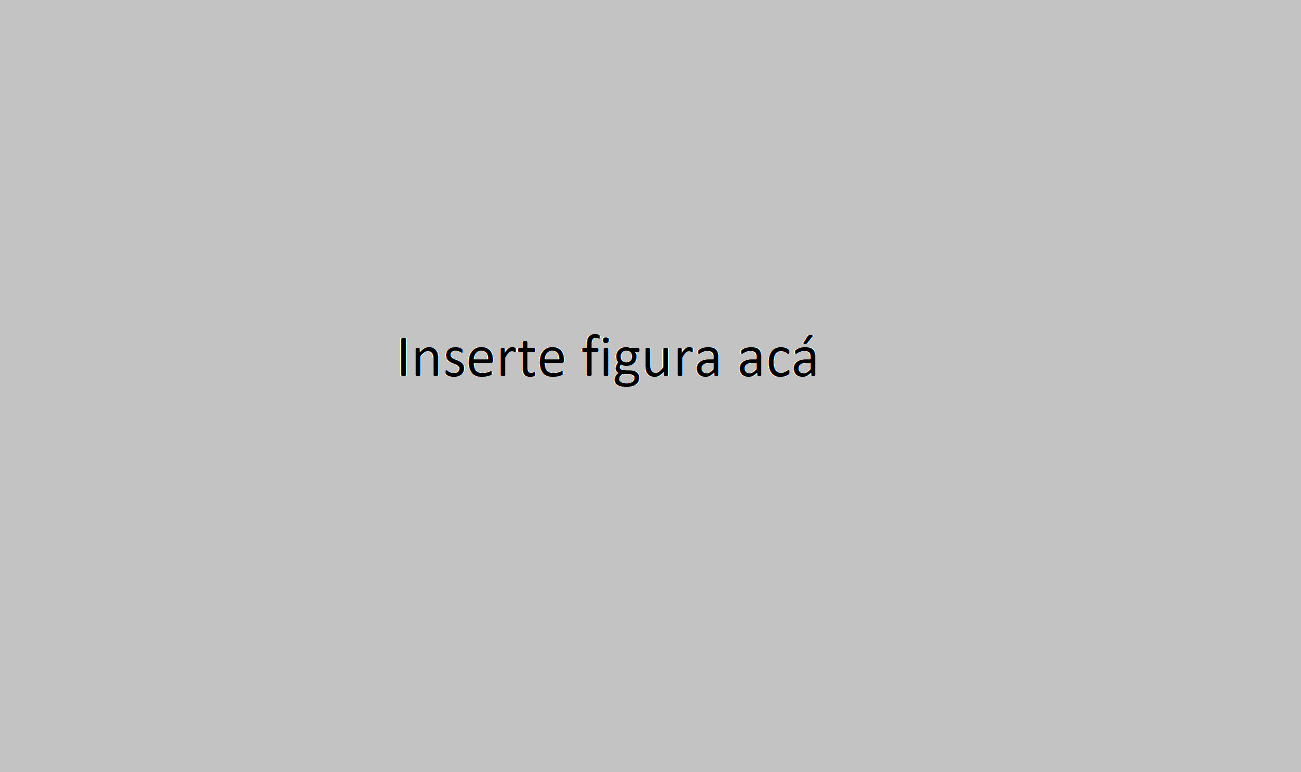
\includegraphics[width=\linewidth]{02_principales/00_figuras/01_figuravacia.png}
\caption{Figura de ejemplo.}
\label{fig_ejemplo}
\end{figure}

\subsection{Planteamiento de Problema}

\lipsum[1-3]

\section{Objetivo General}
\begin{itemize}
    \item \lipsum[10][1-4]
\end{itemize}

\section{Objetivos Específicos}
\begin{enumerate}
    \item \lipsum[10][4-6] 
    \item \lipsum[10][7-11] 
    \item \lipsum[10][10-12]
\end{enumerate}

\section{Justificación}

\lipsum[1-3]

\section{Viabilidad}

\lipsum[5]  

\subsection{Insumos presupuestarios}

\lipsum[5]

\subsection{Insumos tecnológicos}

\lipsum[5]

\subsection{Recursos humanos}

\lipsum[5]

\subsection{Acceso a la información}

\lipsum[5]
\section{Antecedentes del Proyecto}
\subsection{Estudio del Problema a Resolver}

\lipsum[6]

\section{Metodología}

\lipsum[6]

\subsection{Diseño de Investigación}

\lipsum[6]

\subsection{Enfoque de la Investigación}

\lipsum[6]

\subsection{Alcance de la investigación}

\lipsum[6]

\subsection{Limitaciones de la investigación}

\lipsum[6]

\subsection{Cronograma proyectado del desarrollo del proyecto}

\lipsum[6]



\chapter{Marco Teórico}


\section{Sección 1}

\lipsum[6]

\begin{table}[H]
\centering
\caption{Tabla de ejemplo en el marco teórico}
\label{tab_ejemplo}
\begin{tabular}{lccc}
\toprule
\textbf{Descripción}     & \textbf{$r_{0}$} & \textbf{$r_{1}$} & \textbf{$r_{k}$} \\ 
\midrule
Descripción 1 & 0.95 & 0.98 & 1.02 \\
Descripción 2 & 0.97 & 0.99 & 1.02 \\
Descripción 3 & 0.99 & 0.99 & 1.01 \\ 
\bottomrule
\end{tabular}
\end{table}

\begin{equation}
    \text{Costo normalizado} = a + \frac{(c-A)\cdot(b-a)}{(B-A)}
\end{equation}

\subsection{Subsección 1}

\lipsum[7-8]


\chapter{Título Capítulo 3}

\lipsum[5]

\section{Sección 1}

\lipsum[6]

\subsection{Subsección 1}

\lipsum[7]

\subsubsection{subsubsección 1}

\lipsum[8]



\begin{equation*}
E = mc^2    
\end{equation*}

\begin{table}[H]
\centering
\begin{tabular}{llll}
\toprule
Nombre & Edad (años) & Peso (kg) & Altura (m)\\
\midrule
Pedro & 20  & 50 &  1,72\\
Pablo & 39  & 60 &  1,56\\
\bottomrule
\end{tabular}
\caption{}
\label{tab:my-table}
\end{table}


\chapter{Título Capítulo 4}

\lipsum[5]

\section{Sección 1}

\lipsum[6]

\subsection{Subsección 1}

\lipsum[7]

\subsubsection{subsubsección 1}

\lipsum[8]

\chapter{Título Capítulo 5}

\lipsum[5]

\section{Sección 1}

\lipsum[6]

\subsection{Subsección 1}

\lipsum[7]

\subsubsection{subsubsección 1}

\lipsum[8]

\chapter{Conclusiones y Recomendaciones}

\section{Conclusiones}
\begin{enumerate}
    \item \lipsum[8]
    \item \lipsum[9]
\end{enumerate}

\newpage

\section{Recomendaciones}

\begin{enumerate}
    \item \lipsum[11]
    \item \lipsum[8]
\end{enumerate}

%Anexos
\renewcommand{\appendixname}{Anexo}
\renewcommand{\appendixtocname}{Anexo}
\renewcommand{\appendixpagename}{Anexo}

\appendix
\chapter{Título del Anexo A}

\begin{figure}[H]
\centering
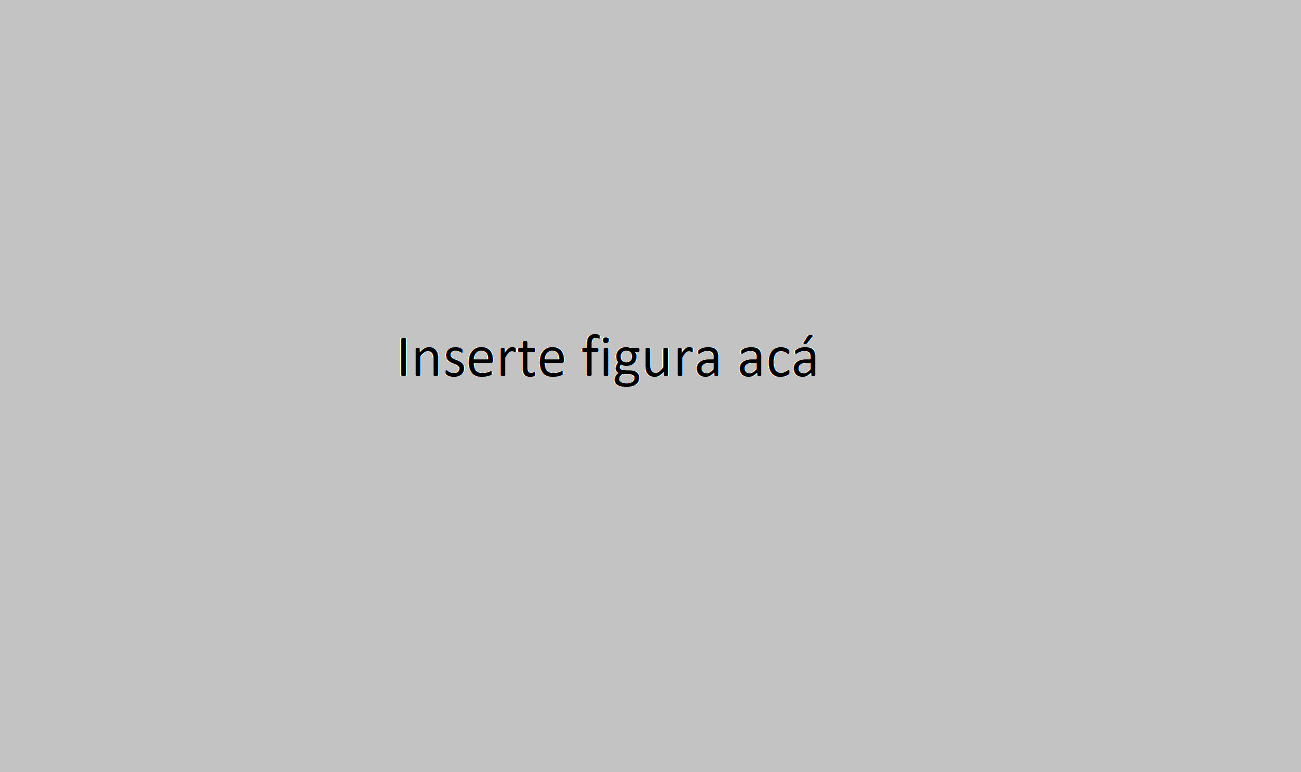
\includegraphics[width=\linewidth]{03_anexos/00_figuras/01_figura.png} % no debe ser mas grande que el texto
\caption{Figura en el Anexo A}
\centering
Fuente:Elaboración propia
\label{fig_a1_ejemplo}
\end{figure}
\chapter{Título del Anexo B}

\begin{figure}[H]
\centering
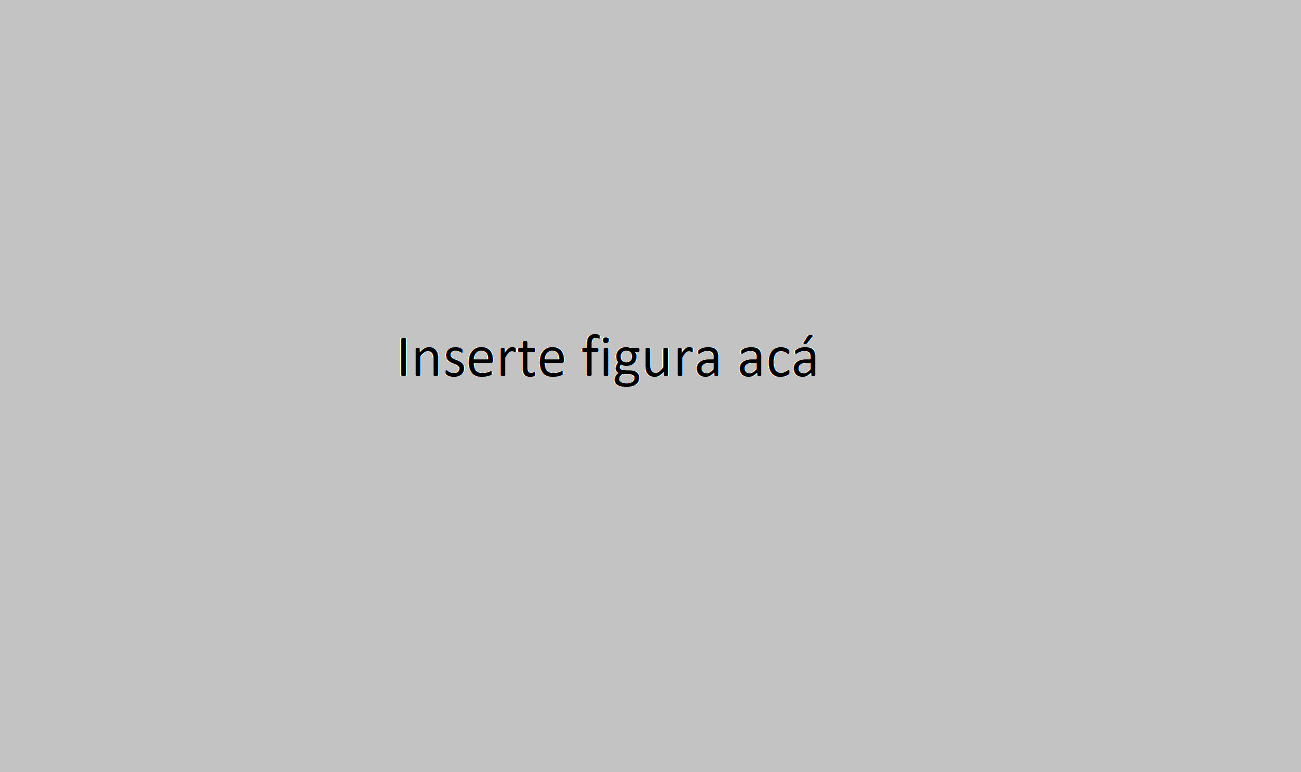
\includegraphics[width=\linewidth]{03_anexos/00_figuras/02_figura.png}
\caption{Figura en el Anexo B}
\centering
Fuente: Elaboración Propia
\label{fig_a2_ejemplo}
\end{figure}
%Apéndices
\renewcommand{\appendixname}{Apéndice}
\renewcommand{\appendixtocname}{Apéndices}
\renewcommand{\appendixpagename}{Apéndices}
\appendix
\thispagestyle{plain}
\chapter*{Hoja de Datos}

\Large
\textbf{Información del Estudiante:}

\normalsize

\textbf{Nombre:} Nombres y Apellidos

\textbf{Cédula:} X-XXXX-XXXX

\textbf{Carné ITCR:} XXXXXXXXXX

\textbf{Dirección de residencia en época lectiva:} Direcció 

\textbf{Teléfono:} XXXX-XXXX

\textbf{Correo electrónico:} email

\vspace{1cm}

\Large
\textbf{Información del Proyecto:}
\normalsize

\textbf{Titulo:} Título

\textbf{Asesor Industrial:} Nombre

\textbf{Profesor Guía:} Nombre

\textbf{Jurado Evaluador:}
\begin{itemize}
    \item Nombre
    \item Nombre
\end{itemize}


\vspace{1cm}
\Large
\textbf{Información de la Empresa:}
\normalsize

\textbf{Nombre:} Nombre

\textbf{Zona:} Región

\textbf{Dirección:} Dirección

\textbf{Actividad principal:} Actividad

\textbf{Contacto:} Nombre y Apellido

\textbf{Teléfono:} XXXX-XXXX


%Bibliografía 
\bibliographystyle{IEEEtran}
\bibliography{Ref}

\end{document}
